\documentclass[conference]{IEEEtran}
\usepackage{times}

% numbers option provides compact numerical references in the text.
\usepackage[numbers]{natbib}
\usepackage{multicol}
\usepackage{graphicx}
\usepackage{subcaption}          % <-- added: the figure block uses subfigure
\usepackage[bookmarks=true]{hyperref}

\newcommand{\newparagraph}[1]{{\bf #1.}}
\usepackage{xcolor}
\definecolor{metaGray}{RGB}{120, 120, 120}
\definecolor{revBlue}{RGB}{0, 114, 178}       % Reviewer A
\definecolor{revOrange}{RGB}{230, 159, 0}     % Reviewer B
\definecolor{revPurple}{RGB}{204, 121, 167}   % Reviewer C
\definecolor{revGreen}{RGB}{0, 158, 115}      % Reviewer D

\newcommand{\AC}{\textcolor{revGreen}{\textbf{AC}}}
\newcommand{\revA}{\textcolor{revBlue}{\textbf{EWFH}}}
\newcommand{\revB}{\textcolor{revOrange}{\textbf{U9qr}}}
\newcommand{\revC}{\textcolor{revPurple}{\textbf{G57g}}}

\begin{document}

\title{Rebuttal  for CoRL Submission \#1342\vspace{-1cm}}
\maketitle
\thispagestyle{empty}

% ---- new-experiment figures, two rows at the top of the page ----
% The whole figure block: two rows across the full width, at the top of the
% rebuttal. Plots first, images second -- the plot row is shorter, so leading
% with it puts the densest quantitative content directly under the opening text.
%
% Widths are chosen so each panel is legible at final size; see
% plot_figures/rebuttal/outputs/final/README.md for the arithmetic.
\begin{figure*}[t]
  \centering
  % Fig 1 -- perception-noise robustness (sim) + real-world failure breakdown.
% Answers: (AC, R1, R2, R3) reliance on pose tracking, and failure analysis.
\begin{subfigure}[t]{0.40\linewidth}
  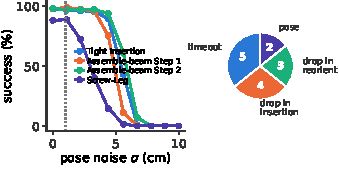
\includegraphics[width=\linewidth]{assets/fig1_noise_and_failures}
  \caption{Success vs.\ object-pose observation noise (left) and the
  breakdown of $14$ real-world failures (right).}
  \label{fig:noise_failures}
\end{subfigure}
\hfill
  % Fig 4 -- free-standing (unbolted) fixtures, same policy, no retraining.
% Answers: (AC, R3) dependence on fixed fixtures.
\begin{subfigure}[t]{0.30\linewidth}
  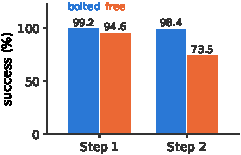
\includegraphics[width=\linewidth]{assets/fig4_unbolted_fixture}
  \caption{Bolted vs.\ free fixture, no retraining.}
  \label{fig:unbolted}
\end{subfigure}
\hfill
  % Fig 5 -- one co-trained policy vs. per-task policies.
% Answers: (AC, R2, R3) "the downstream policies are task-specific".
\begin{subfigure}[t]{0.30\linewidth}
  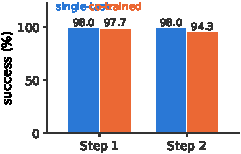
\includegraphics[width=\linewidth]{assets/fig5_unified_policy}
  \caption{A single co-trained policy matches per-task policies.}
  \label{fig:unified}
\end{subfigure}


  \vspace{2pt}

  % Fig 3 -- novel / complex task geometries at real-world scale.
% Answers: (AC, R2, R3) enlarged and limited task geometries, and R2's
% "naturally sized electric plug" by name.
% Dimensions come FIRST so the reader establishes scale before seeing the
% rollout: the objection is that the parts are enlarged, not that they fail.
\begin{subfigure}[t]{0.62\linewidth}
  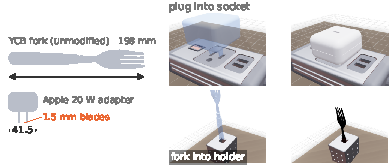
\includegraphics[width=\linewidth]{assets/fig3_novel_geometries}
  \caption{Two real-world-scale tasks. The plug is compact with $1.5$\,mm
  blades and is a two-feature insertion; the fork is an unmodified YCB scan.}
  \label{fig:novel_geometries}
\end{subfigure}
\hfill
  % Fig 2 -- real-world END-TO-END beam assembly, 20 trials.
% Answers: (AC, R3) extended real-world trials; the paper evaluated Step 1 and
% Step 2 separately, this runs both in sequence.
\begin{subfigure}[t]{0.38\linewidth}
  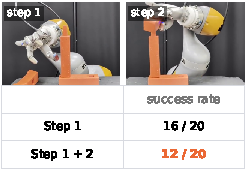
\includegraphics[width=\linewidth]{assets/fig2_end_to_end}
  \caption{End-to-end two-step beam assembly, $20$ real-world trials.}
  \label{fig:end_to_end}
\end{subfigure}

  \vspace{-6pt}
\end{figure*}


We thank the reviewers and AC for their thoughtful and \textit{unanimously} positive feedback. They recognize that \textit{Play2Perfect} tackles an ``important and challenging robot-learning problem'' (\revB, \revC) with a ``well-motivated and intuitive solution" (\AC, \revA, \revB), presents ``rigorous and systematic ablations" yielding ``clear, actionable, and useful insights" (\AC, \revA, \revB, \revC), achieves ``large efficiency gains" over RL training from scratch (\AC, \revA, \revB), and demonstrates ``impressive zero-shot real-world results" (\AC, \revA, \revB, \revC). We now address their questions:

% ------------------------------------------------------------------
% Answers go here. Figure references available:
%   \ref{fig:noise_failures}   \ref{fig:end_to_end}
%   \ref{fig:novel_geometries} \ref{fig:unbolted}  \ref{fig:unified}
% ------------------------------------------------------------------

\end{document}
